\section{Resultados}
Realizando la simulación del sistema bajo los parámetros usados en la tabla \ref{table:parametros} se obtuvó que la energía total de cada sistema
se encuentra en un estado oscilatorio, para cada densidad es diferente el valor al cual oscila y en situaciones la energía llega a subir, pero nuevamente 
decae y vuelbe a oscilar. Esto se puede apreciar en la figura \ref{fig:energiatotal}.
\begin{figure}[H]
    \centering
    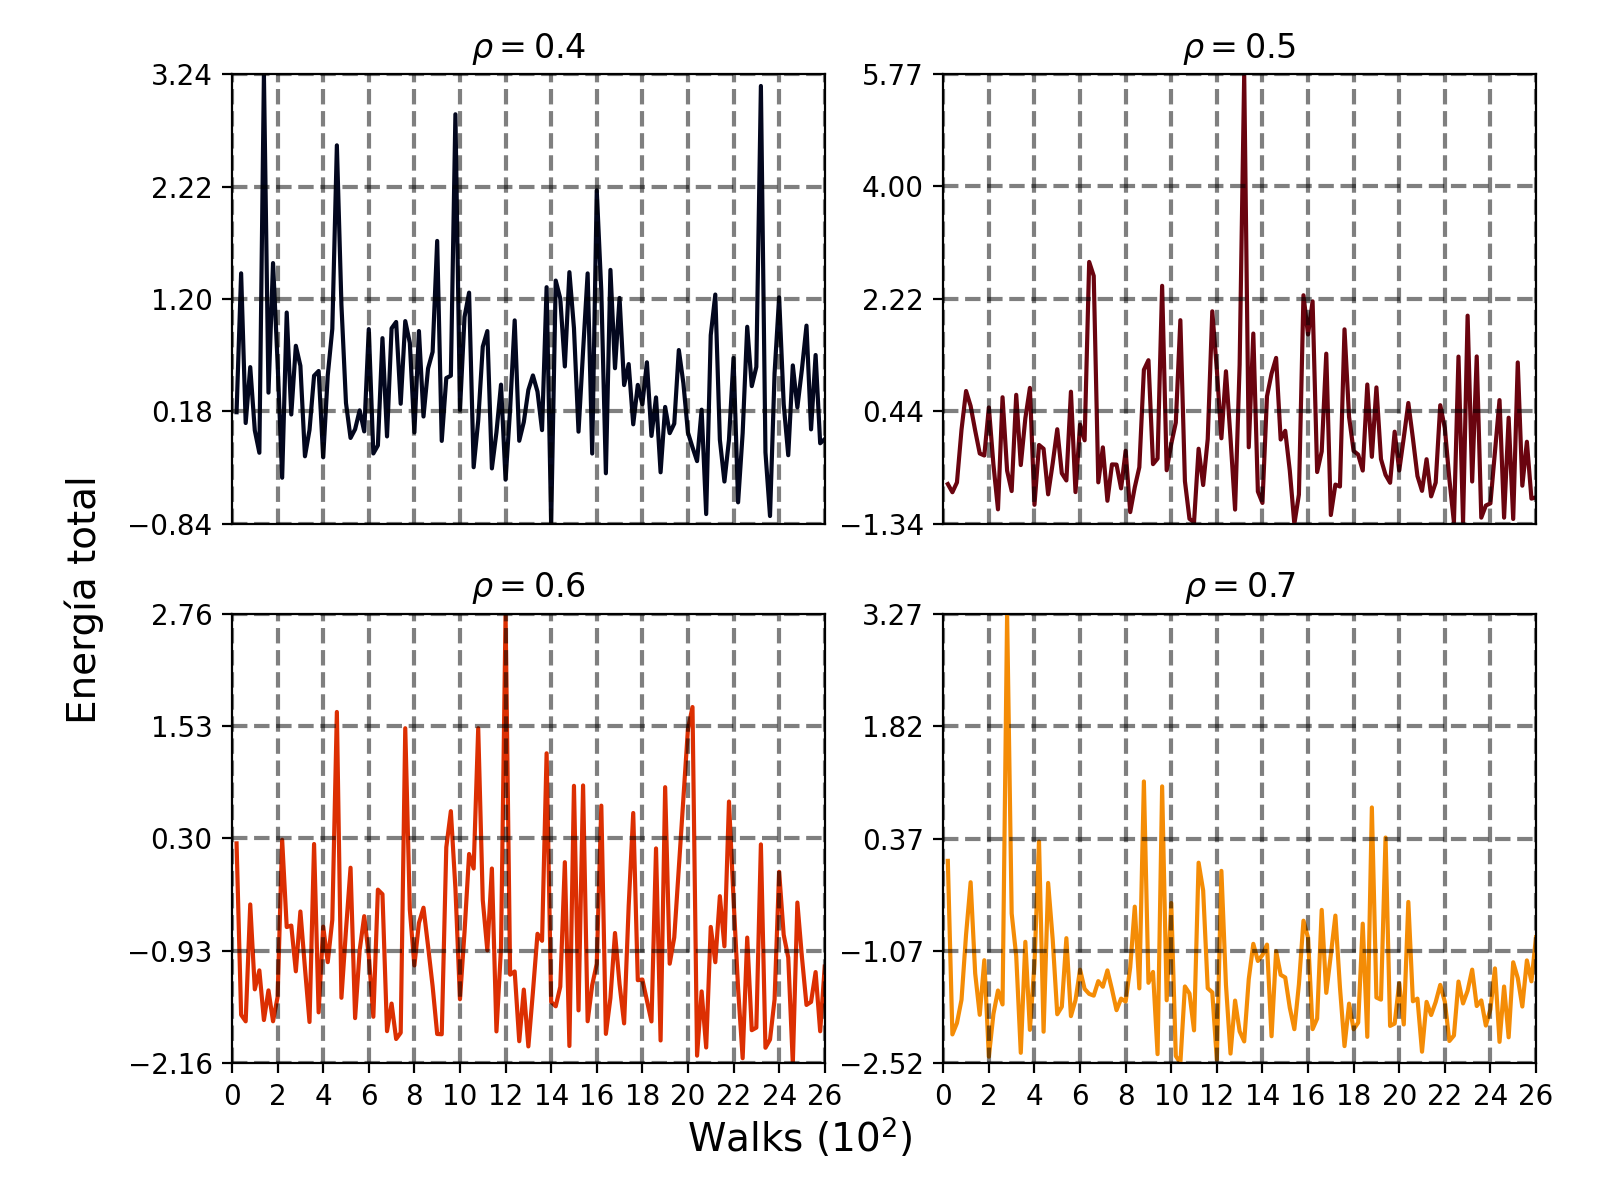
\includegraphics[scale=0.35]{../Graphics/Energy.png}
    \caption{Energía total del sistema a lo largo de la simulación para las densidades utilizadas.}
    \label{fig:energiatotal}
\end{figure}
Al estar calculando la energía cinetica y potencial del sistema, se pudo obtener la temperatura a cada paso de la simulación. En la figura
\ref{fig:temp} se aprecia como la temperatura toma un valor constante a lo largo de la simulación realizando pequeñas fluctuaciones alrededor
de un valor, en este caso todas alrededor de $T=2$.
\begin{figure}[H]
    \centering
    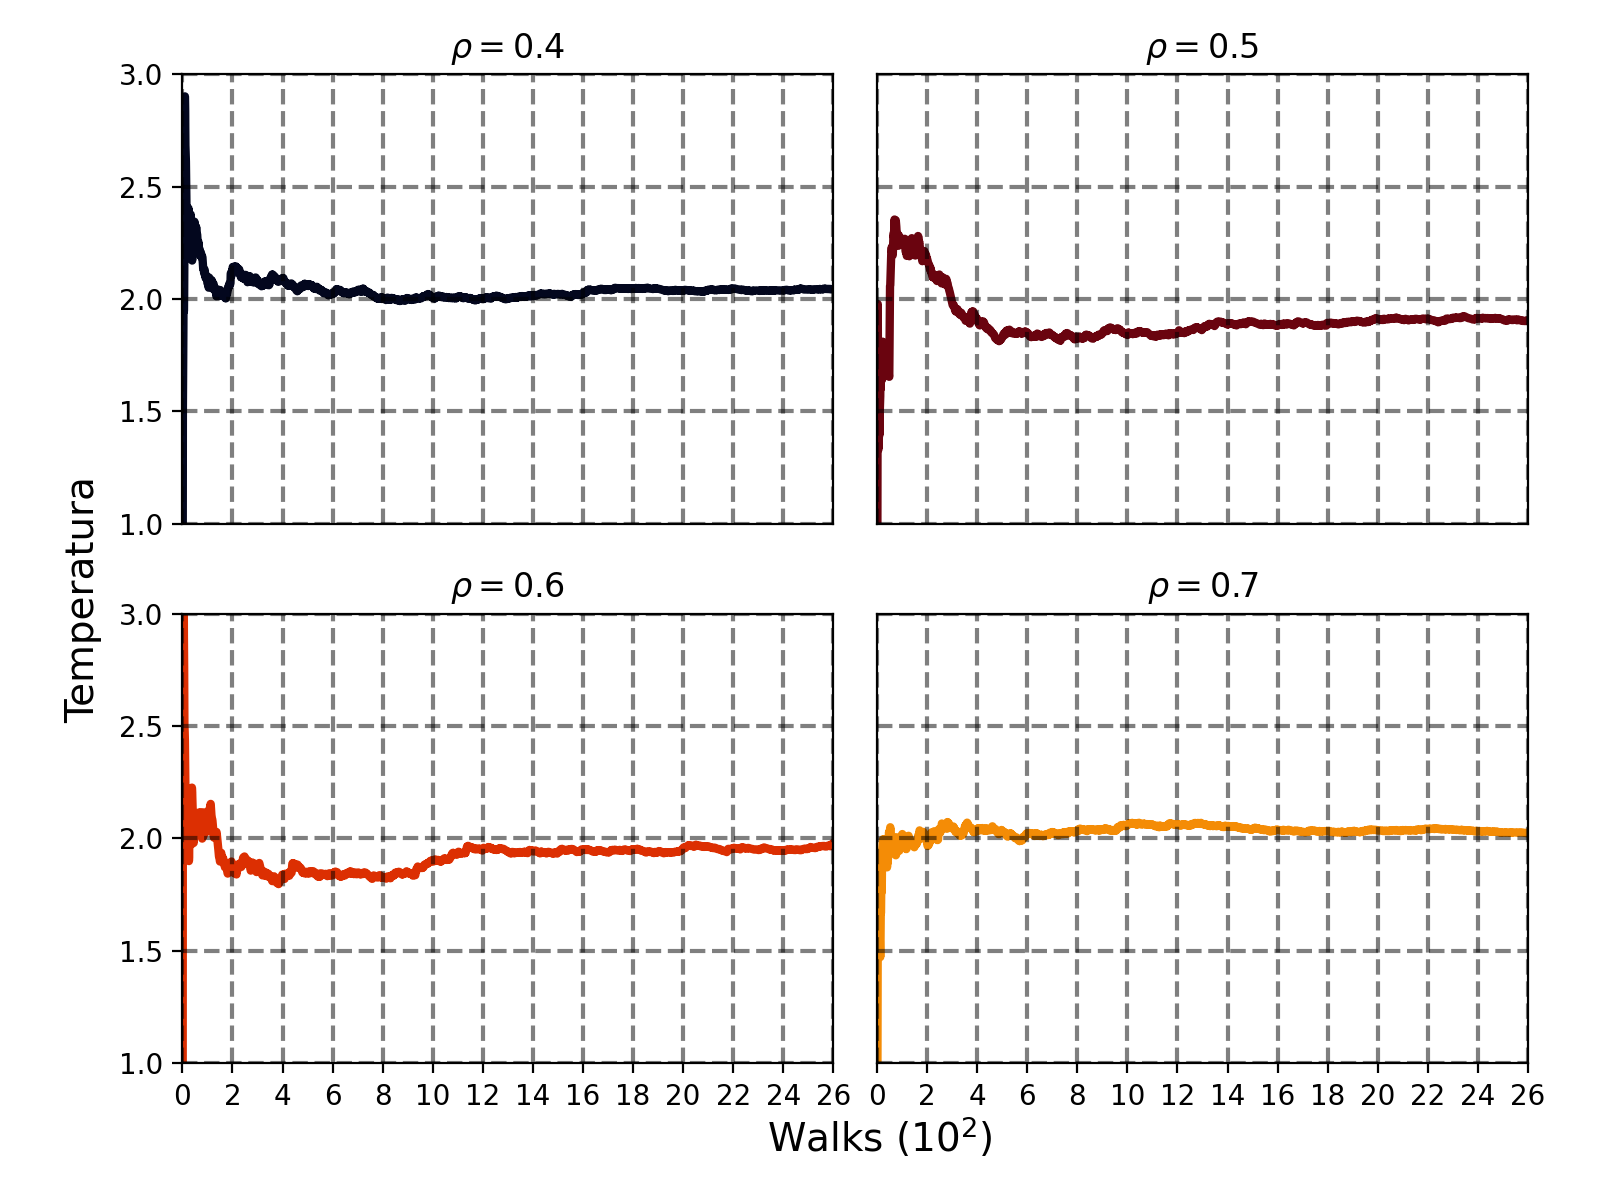
\includegraphics[scale=0.35]{../Graphics/Temp.png}
    \caption{Temperatura del sistema a lo largo de la simulación para las densidades utilizadas.}
    \label{fig:temp}
\end{figure}
Del mismo proceso, se obtuvo la figura \ref{fig:temp} la cual muestra la distribución radial del sistema para las diferentes densidades usadas para la simulación, 
en esta se puede observar que los átomos tienden a estar a una distancia cercana entre todos, en las mismas distribuciones se aprecia que presenta
fluctuaciones a diferentes distancias.
\begin{figure}[H]
    \centering
    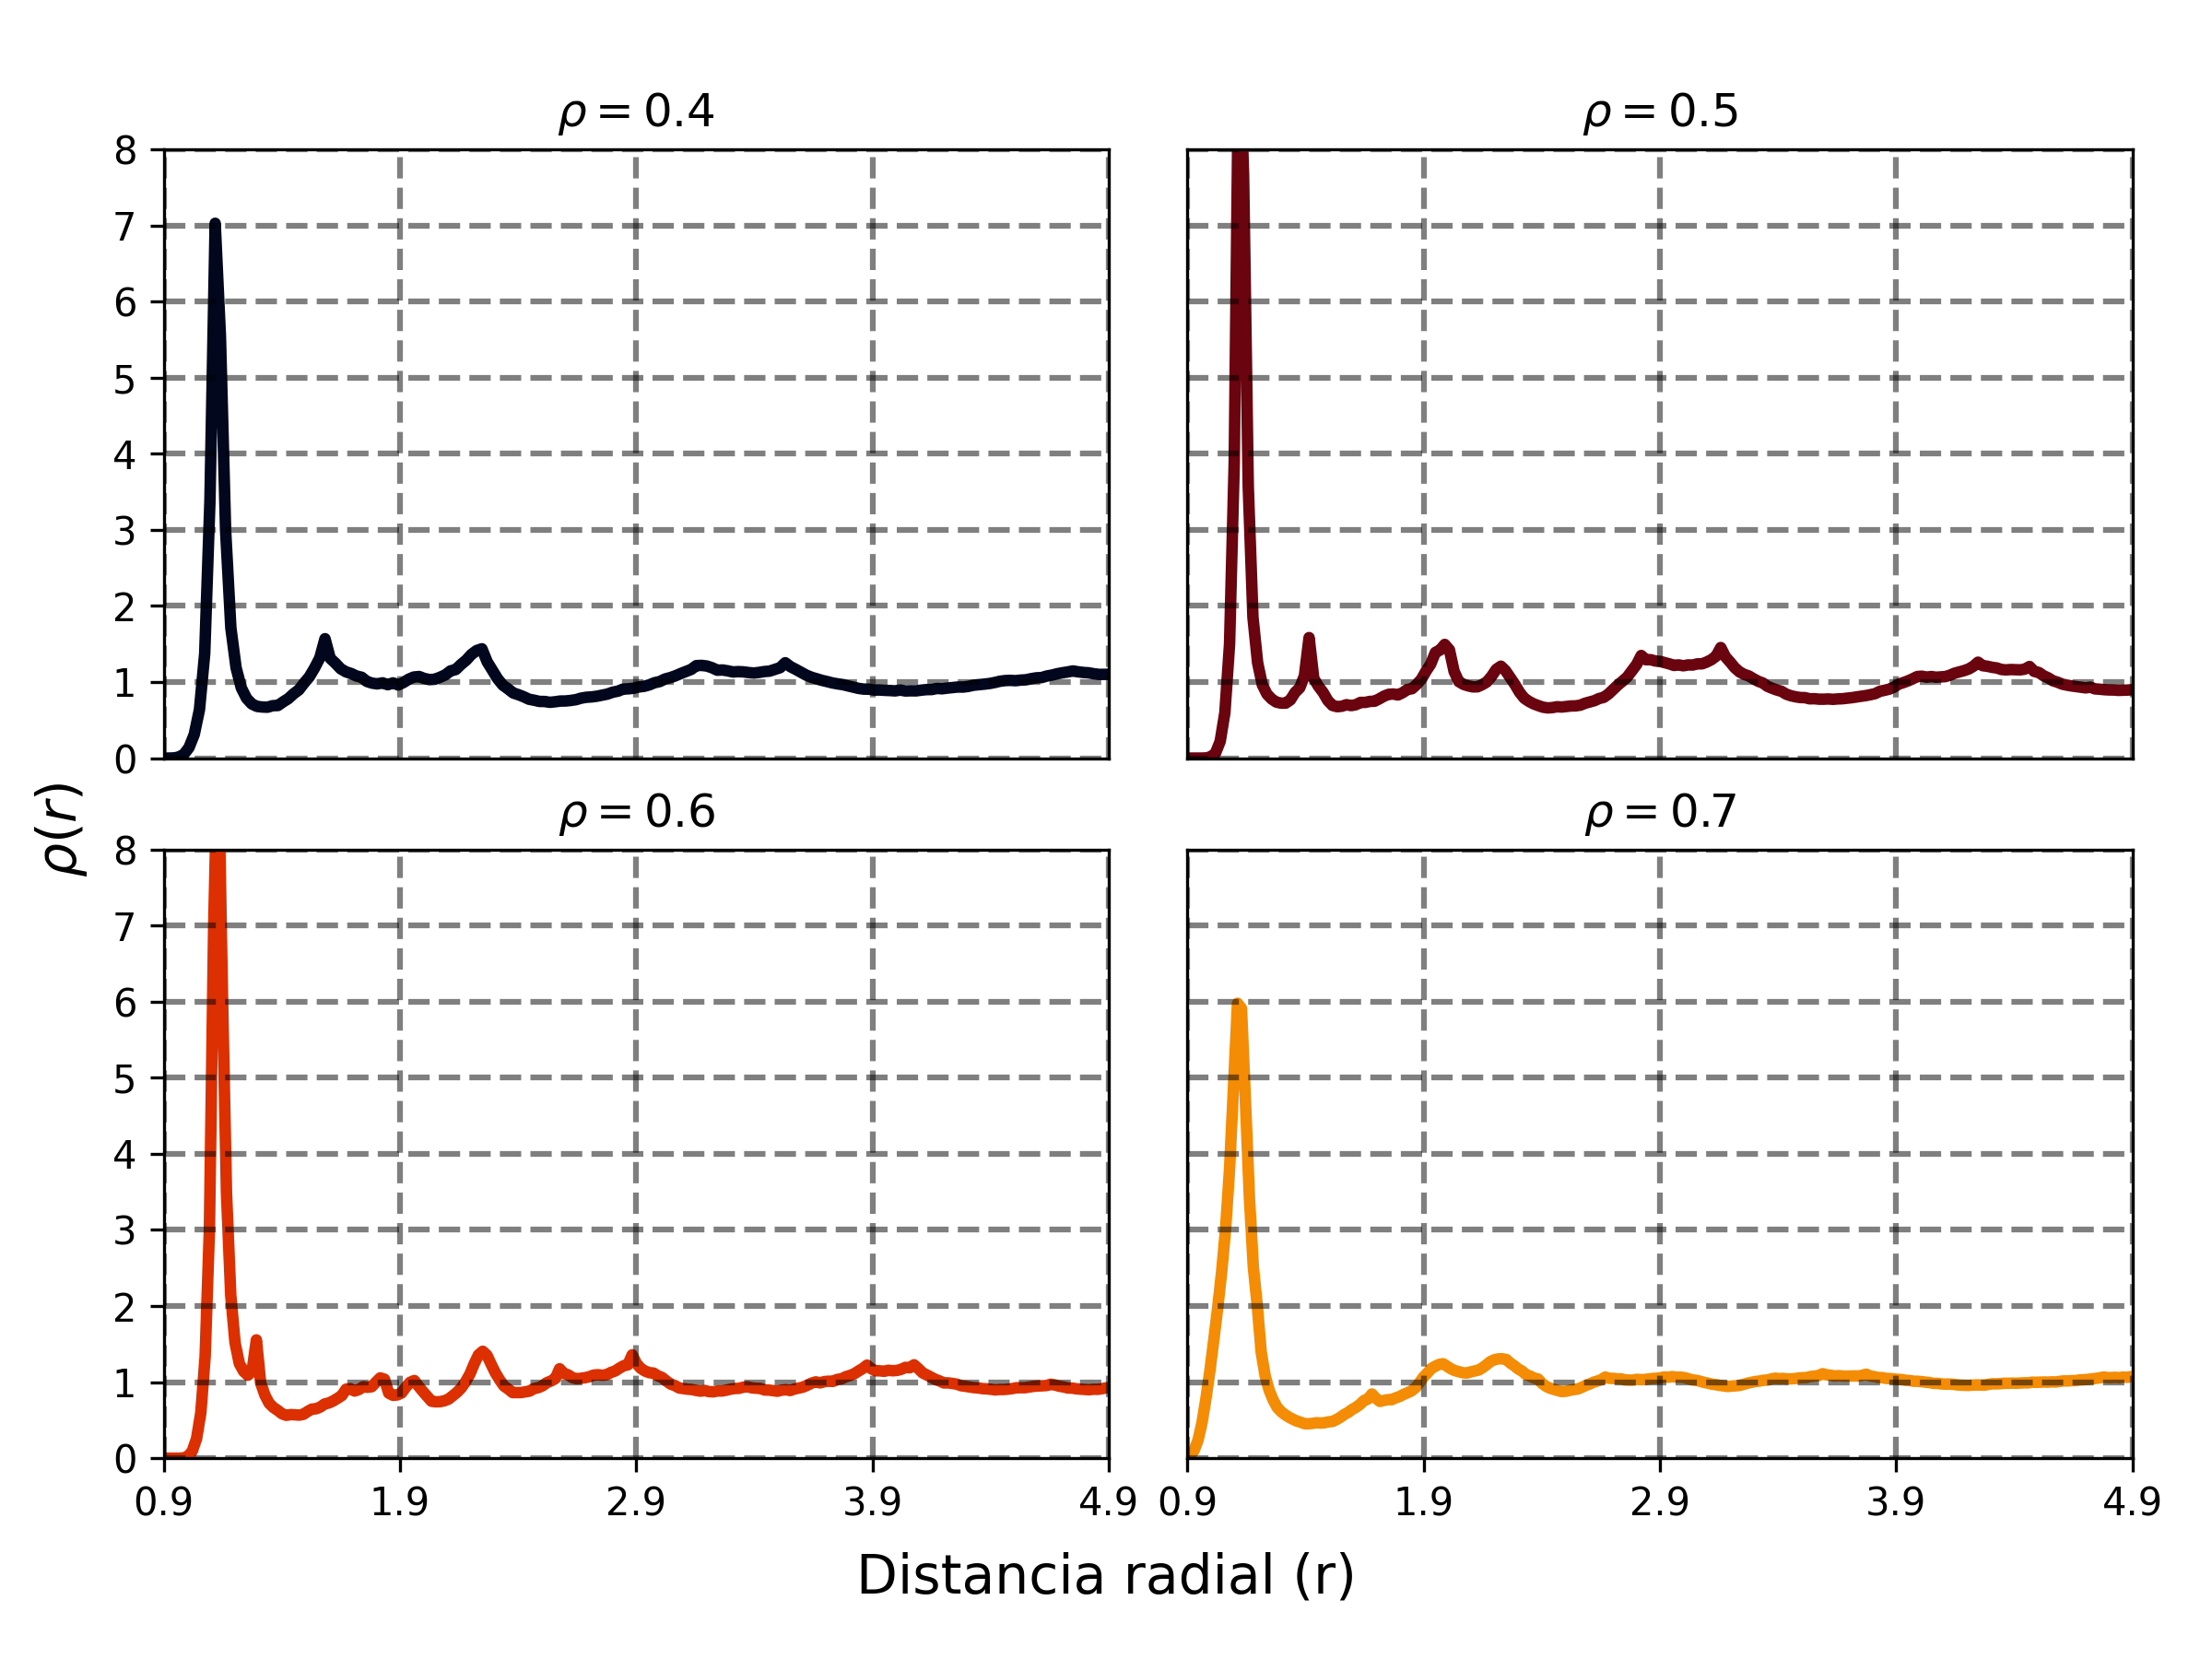
\includegraphics[scale=0.35]{../Graphics/Dis_rad.png}
    \caption{Distribución radial del sistema obtenida para las densidades utilizadas.}
    \label{fig:disrad}
\end{figure}
Durante la simulación se grabaron las velocidades en x y y de todas las partículas, por lo que al agruparlas en un arreglo, uno para cada densidad, se obtuvo
la figura \ref{fig:disvel}. A cada conjunto de velocidades se le realizó un fit con la distribución normal, mostrando asi que estas velocidades
se encuentran dentro de una distribución normal. 
\begin{figure}[H]
    \centering
    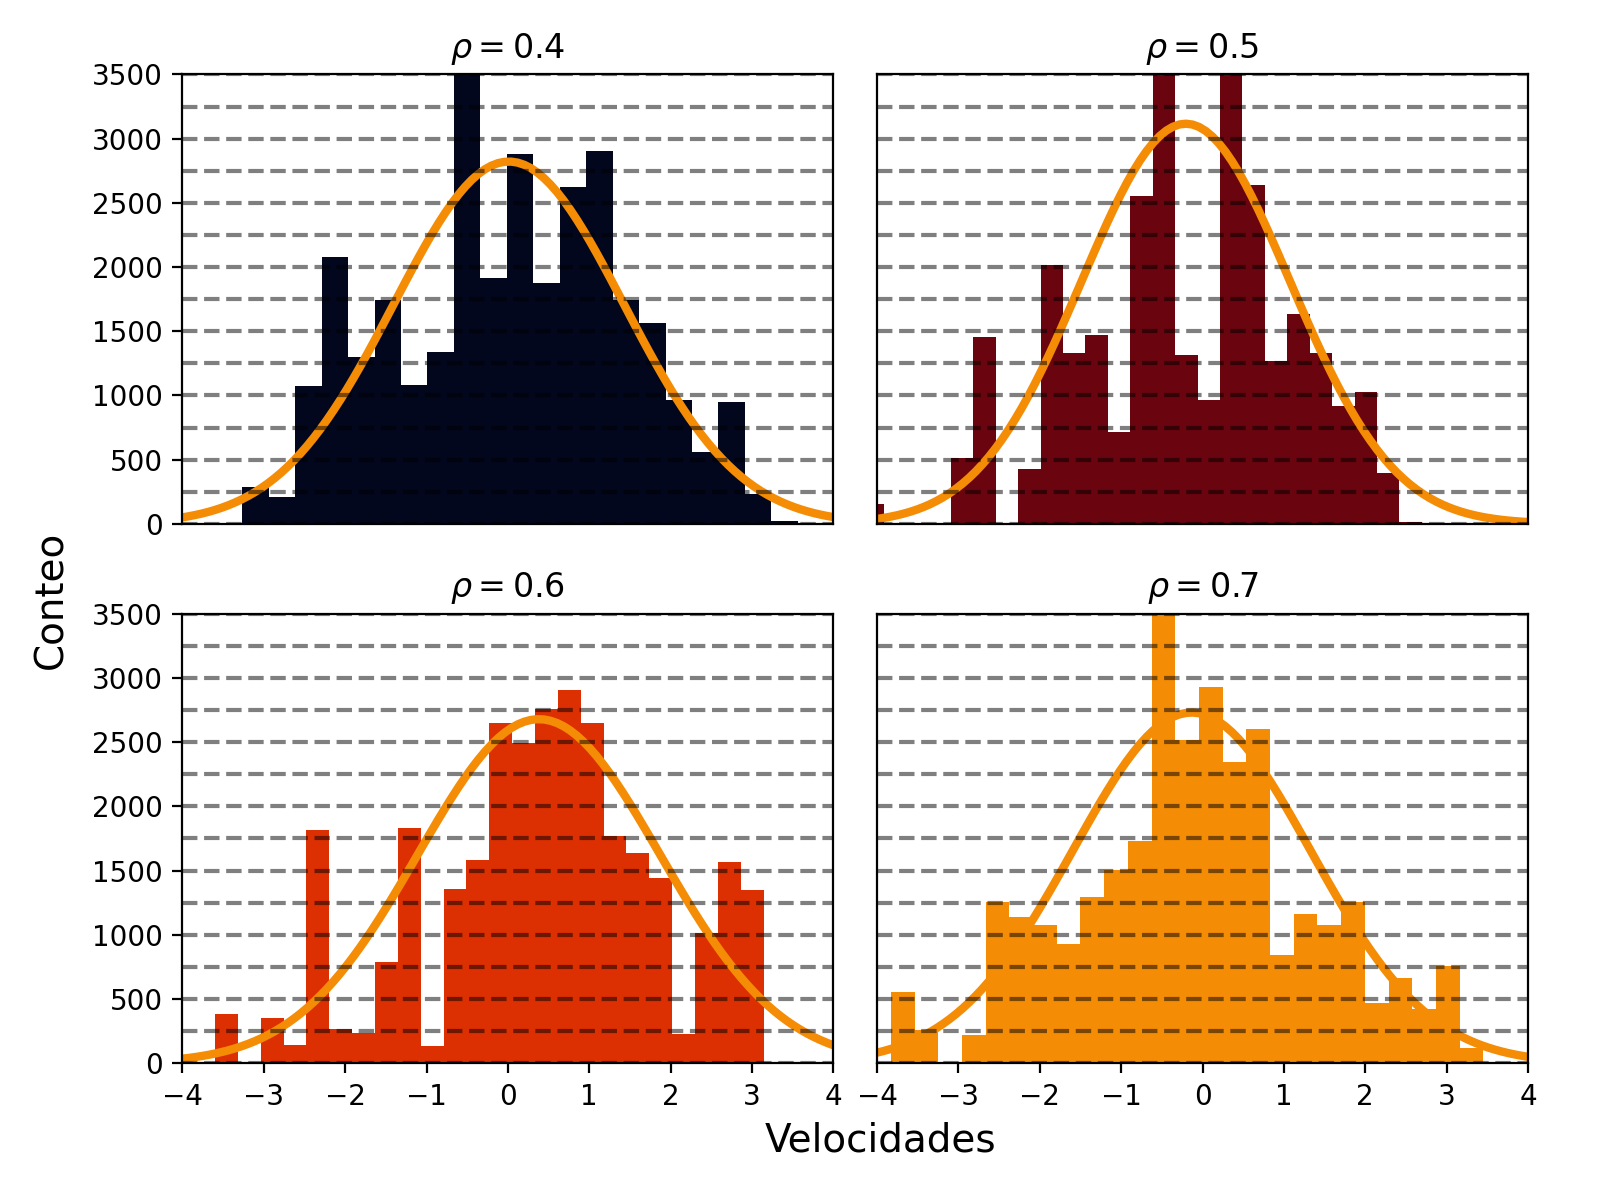
\includegraphics[scale=0.35]{../Graphics/vel.png}
    \caption{Distribución de las velocidades de los diferentes sistemas junto con un fit de una distribución normal.}
    \label{fig:disvel}
\end{figure}